\chapter{Análise dos Eventos de Calorimetria}
\label{chap:dados}

Neste capítulo, serão apresentados os conjunto de dados utilizados para o desenvolvimento da pesquisa proposta. Adicionalmente, serão apresentadas as técnicas utilizadas para o pré-processamento inicial destes dados, antes de serem efetivamente utilizados para estudo. Estudos serão apresentados para identificar as principais características dos eventos a serem discriminados, bem como para validar que não apresentam problemas que inviabilizem sua utilização.

\section{Geração dos Eventos}
\label{sec:geracao_eventos}

Os eventos utilizados neste trabalho são oriundos de simulações de Monte Carlo ***REF*** produzidas pelos próprios colaboradores do ATLAS utilizando o \emph{Pythia} e o \emph{Geant}, e que ficam disponíveis para análise. ***FALAR O QUE TEM NESSES DADOS (PRE-FILTRADOS PELO LVL1, BYTE STREAM JA FEITO, OU SEJA, COMPARANDO COM A FAQUISICAO REAL DE DADOS, ESTES EVENTOS SIMULAM QUAL PONTO?)***. A tabela~\ref{tab:datasets} apresenta as informações dos conjuntos utilizados. São apresentados o nome de cada conjunto, conforme nomenclatura definida em ***REF***. 

\begin{table}
\caption{Informações dos eventos utilizados para análise.}
\begin{center}
{\tiny
\begin{tabular}{|l|l|l|l|l|}
\hline
\textbf{Conjunto} & \textbf{Tipo} & \textbf{\emph{Pile-up}} & \textbf{Energia (Gev)} & \textbf{Quantidade} \\
\hline
mc08.107020.singlepart\_e\_Et7-80.digit.RDO.e342\_s439 & Elétrons simples & Não & 7-80 & X \\
\hline
misal1\_mc12.005802.JF17\_pythia\_jet\_filter.digit.RDO.v12003105 & Di-jatos & Não & Y & X \\
\hline
ideal2\_mc12.005011.J2\_pythia\_jetjet.digit.RDO.v13003004 & Di-jatos & Não & Y & X \\
\hline
ideal2\_mc12.005012.J3\_pythia\_jetjet.digit.RDO.v13003004 & Di-jatos & Não & Y & X \\
\hline
\end{tabular}
}
\end{center}
\label{tab:datasets}
\end{table} 

Para o desenvolvimento de sistemas de filtragem elétron / jato para o segundo nível de filtragem do ATLAS, estes eventos precisam, inicialmente serem pré-filtrados pelo primeiro nível, para que os estudos sejam realizados somente nos eventos que, de fato, chegarão ao segundo nível. Para tal, utilizou-se o Athena para emular o primeiro nível de filtragem, para que este isolasse as regiões de interesse a serem propagadas ao segundo nível. Para que o conjunto resultante da filtragem contenha a maior quantidade possível de especificidades, um corte de baixa energia (7 Gev) foi utilizado, sendo este limiar de corte recomendado pela colaboração ATLAS para análises. Adicionalmente, o LVL1 foi configurado para não observar o vazamento de energia para a camada hadrônica (cortes sem isolamento). Desta maneira, o conjunto de RoI resultante conteria eventos de todas as assinaturas geradas pelo LVL1. Uma vez selecionadas,  as RoI foram copiadas para um arquivo em disco para que pudessem ser analisadas \emph{offline}. É apresentado na tabela~\ref{tab:num_eventos_filtrados}  o número final de regiões de interesse obtidas ao final do processo de pré-filtragem pelo LVL1\footnote{Os números apresentados são os totais por tipo de partícula, independente do conjunto de origem.}.

\begin{table}
\caption{Número de RoI obtidas para cada padrão após filtragem pelo LVL1.}
\begin{center}
\begin{tabular}{|l|l|}
\hline
\textbf{Padrão} & \textbf{Total de Eventos} \\
\hline
Elétron & 470.282 \\
\hline
Jato &  1.366.548 \\
\hline
\end{tabular}
\end{center}
\label{tab:num_eventos_filtrados}
\end{table} 

A figura~\ref{fig:estatistica_inicial}, são apresentados os histogramas de energia transversa total de cada RoI, além dos valores de $\eta$, $\phi$ e dos códigos dos detetores de cada célula. Para a distribuição de energia, consideramos apenas o espectro de energia na faixa de $7 \le E_T \le 80$ Gev, visto que é nesta região que se encontram as principais assinaturas de eventos eletromagnéticos. Para a distribuiçào em $\eta$, a análise desconsiderou a parte interna da tampa e o \emph{forward calorimeter}, visto que a probabilidade de eventos interessantes nesta região é bastante reduzida ***REF***.  No caso da distribuição em $\phi$, observa-se que  as células cobrem toda a faixa entre $\pm \pi$, permitindo a análise do peculiar caso onde o centro da RoI fica perto da região de $\pm \pi$ (\emph{phi-wraparound}). Por fim, a distribuição de células pelas camadas de cada calorímetro mostra que todos os subdetetores, com exceção do \emph{forward calorimeter} foram considerados. A linha tracejada apresentada indica qual seria o valor esperado do número de celulas em cada camada, considerando o tamanho de cada célula. Por exemplo, a primeira camada eletromagnética (\texttt{EM1}), na região do barril,  possui células cujo tamanho é a metade das células na segunda camada eletromagnética (\texttt{EM2}), para a mesma região, de tal forma que devemos encontrar, aproximadamente o dobro do numero de células em (\texttt{EM1}) do que em (\texttt{EM2}), como confirma a figura~\ref{fig:estatistica_inicial}. ***EXPLICAR POR QUE O PSENDCAP TEM MUITO MENOS CELULAS QUE O ESPERADO E O GAPSCI0 TEM MUITO MAIS CELULAS DO QUE O ESPERADO***

\begin{figure}
\centering 
\subfloat[Elétrons]{\label{fig:estatistica_inicial_eletrons} 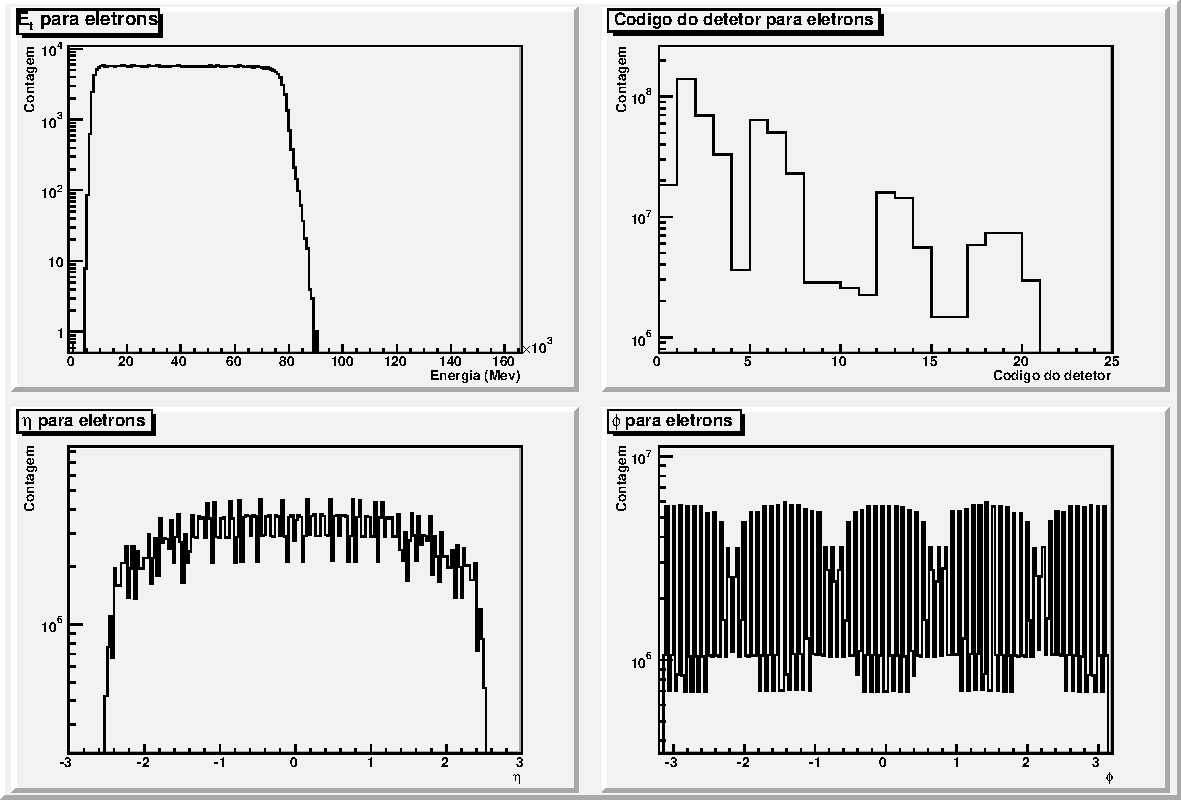
\includegraphics[height = 7cm]{hist_et_det_eta_phi_for_electrons}} \\
\subfloat[Jatos]{\label{fig:estatistica_inicial_jatos} 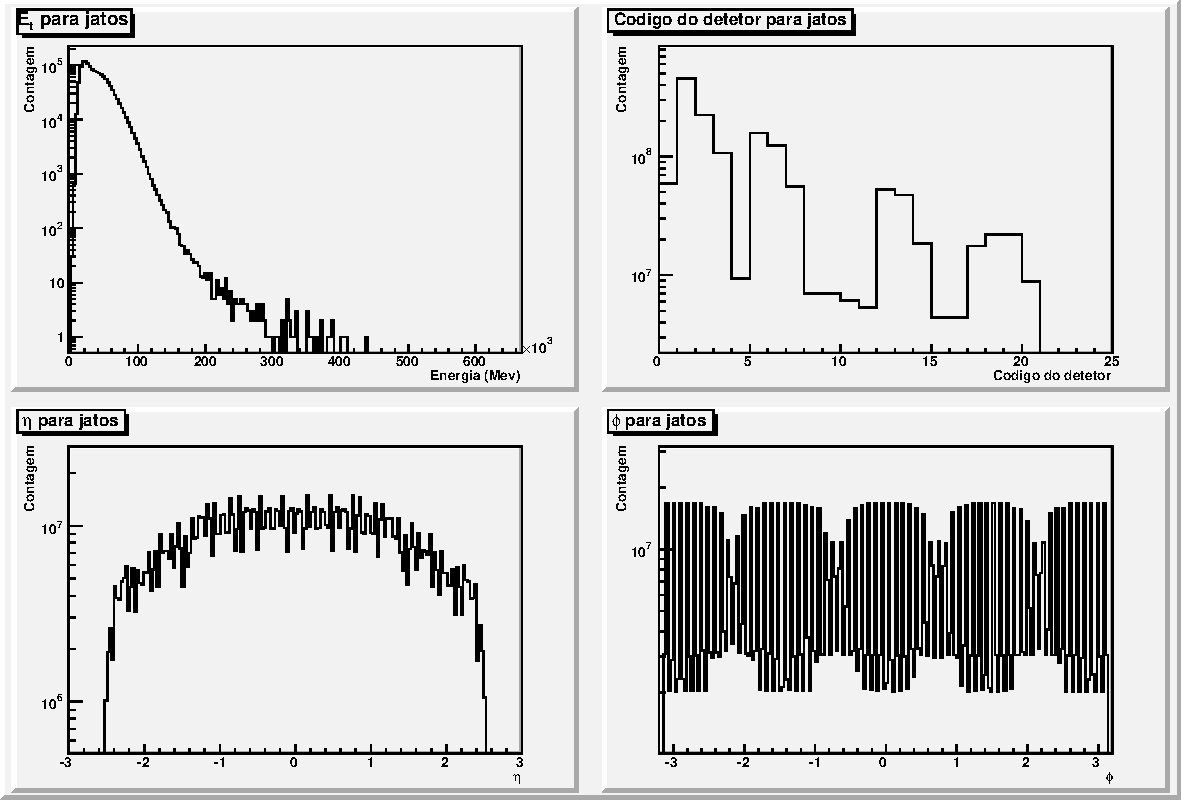
\includegraphics[height = 7cm]{hist_et_det_eta_phi_for_jets}}
\caption{Distribuição da informação proveniente dos calorímetros para cada tipo de partícula.} 
\label{fig:estatistica_inicial} 
\end{figure} 


Outra análise importante para a validação destes eventos é o vazamento de energia para a seção hadrônica de calorimetria. É apresentada na figura~\ref{fig:energia_secao_hadronica} a distribuição, em valores percentuais, da energia absorvida pela seção hadrônica de calorimetria, comparada com a energia total da RoI. Como esperado, temos que, na média, jatos depositam um percentual maior de sua energia na seção hadrônica. Grandes percentuais de energia podem ser observados para jatos, na figura~\ref{fig:energia_secao_hadronica_jatos}, o que é esperado, visto que a assinatura usada no  primeiro nível para a filtragem destes eventos não utilizava o vazamento de energia para a seção hadrônica como parâmetro de corte (corte sem isolamento). Por outro lado,  os altos ($\ge 10\%$) valores de energia na seção hadrônica apresentados na figura~\ref{fig:energia_secao_hadronica_eletrons} para elétrons requerem uma análise mais profunda, visto que a seção eletromagnética foi concebida para absorver totalmente a energia de eventos eletromagnéticos. 

\begin{figure}
\centering 
\subfloat[Elétrons]{\label{fig:energia_secao_hadronica_eletrons} \includegraphics[height = 5cm]{percentual_energia_secao_hadronica-eletrons}}
\subfloat[Jatos]{\label{fig:energia_secao_hadronica_jatos} \includegraphics[height = 5cm]{percentual_energia_secao_hadronica-jatos}}
\caption{Distribuição do percentual de energia depositada na seção hadrônica.} 
\label{fig:energia_secao_hadronica} 
\end{figure} 

Pode ser observado na figura~\ref{had_sec_analysis-all_detectors} a análise mais detalhada para os elétrons que depositam mais de 10\% de sua energia total na seção hadrônica. Como esperado, esta variação não tem relação com a posição em $\phi$ da partícula, como fica evidente observando-se a distribuição desta grandeza. O gráfico com a variação da energia depositada na seção hadrônica em relação à energia total da RoI mostra uma ascensão linear da concentração na seção hadrônica, o que é um comportamento esperado. Os eventos com energia hadrônica negativa são aqueles que não ultrapassaram o limiar de ruído, ficando com valores negativos após a subtração do pedestal de ruído. A distribuição em $\eta$, por sua vez, indica as causas  deste fenômeno. Primeiramente, temos a concentração em $| \eta | \sim 0$, que é resultado da existência de uma fenda na região $| \eta < 0.015 |$ existente apenas no calorímetro eletromagnético, de tal forma que a absorção de energia nesta região, para o calorímetro eletromagnético fica bastante reduzida. A segunda região com grande concentração de eventos é a região  com $1,475 \leq | \eta | \leq 1,6$, correspondente à zona da fenda do calorímetro eletromagnético, de tal forma que grande parte da energia dos eventos nesta região é depositada nos cintiladores colocados nesta faixa (vide figura~\ref{fig:deposicao_energia_cintiladores}), que, na análise realizada, contam como energia hadrônica. Por fim, observa-se que muito dos eventos estão na região da tampa ***EXPLCIAR PQ ESTAO NA REGIAO DA TAMPA***

\begin{figure}
\centering 
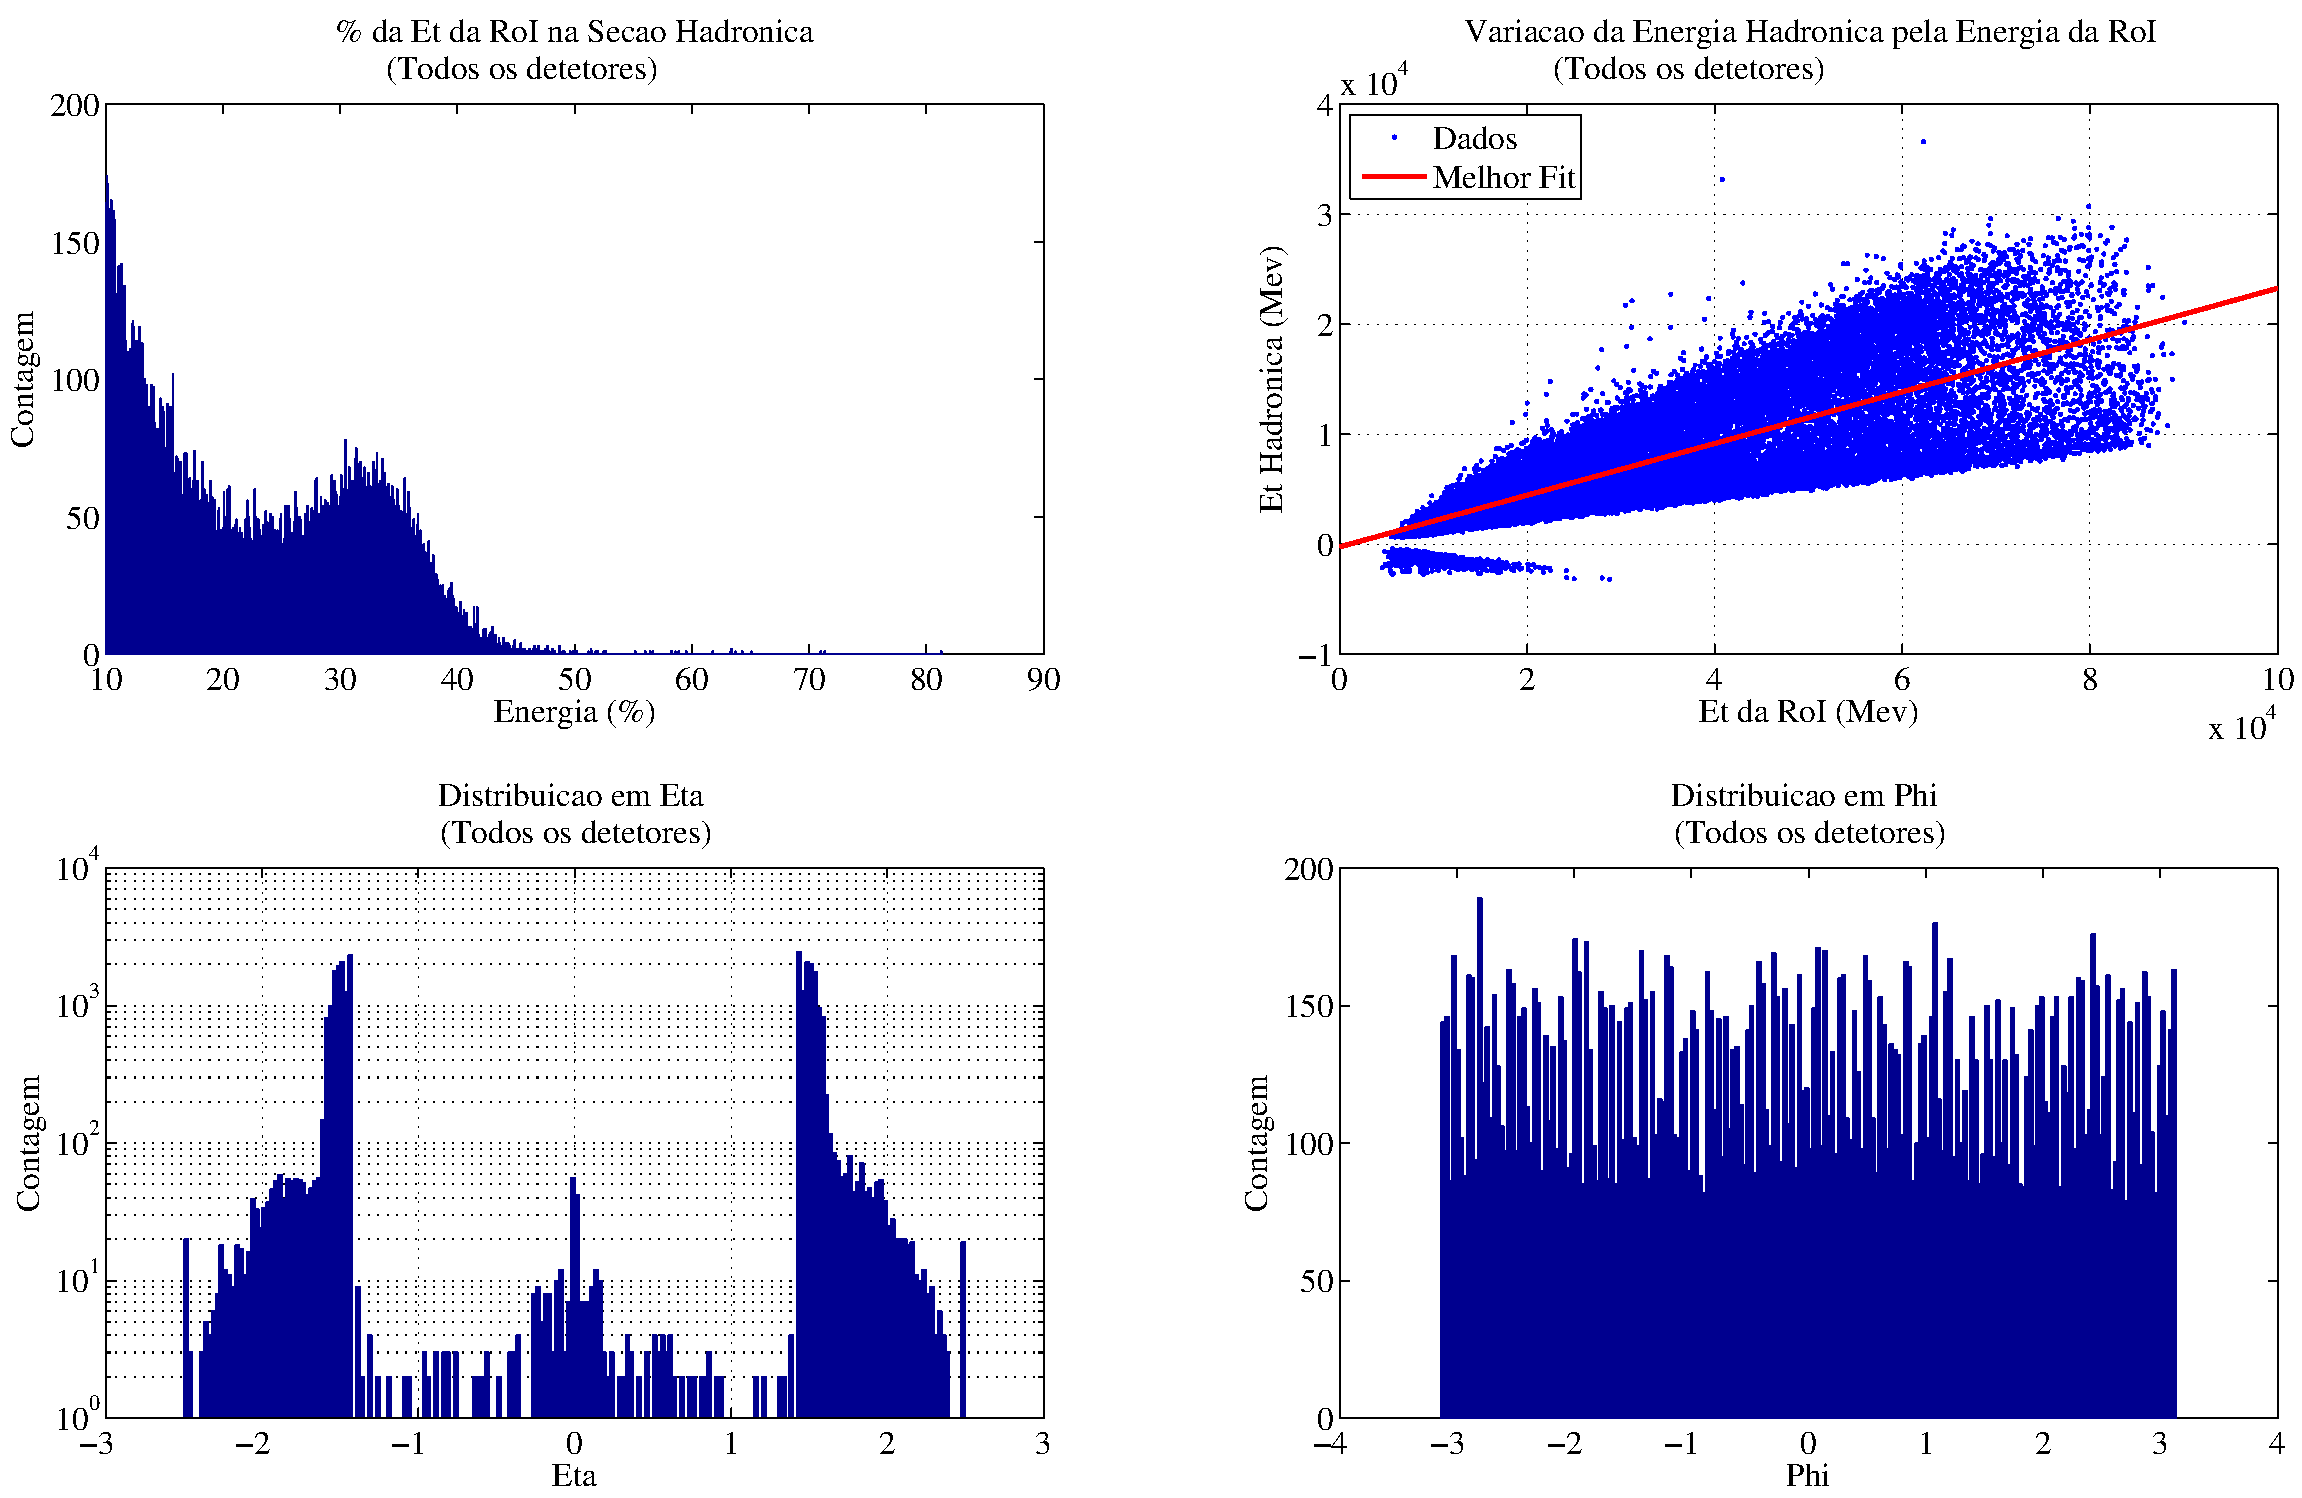
\includegraphics[height = 7cm]{had_sec_analysis-all_detectors}
\caption{Análise da alta deposição de energia na seção hadrônica para elétrons.} 
\label{fig:analise_secao_hadronica_eletrons} 
\end{figure} 


\begin{figure}
\centering 
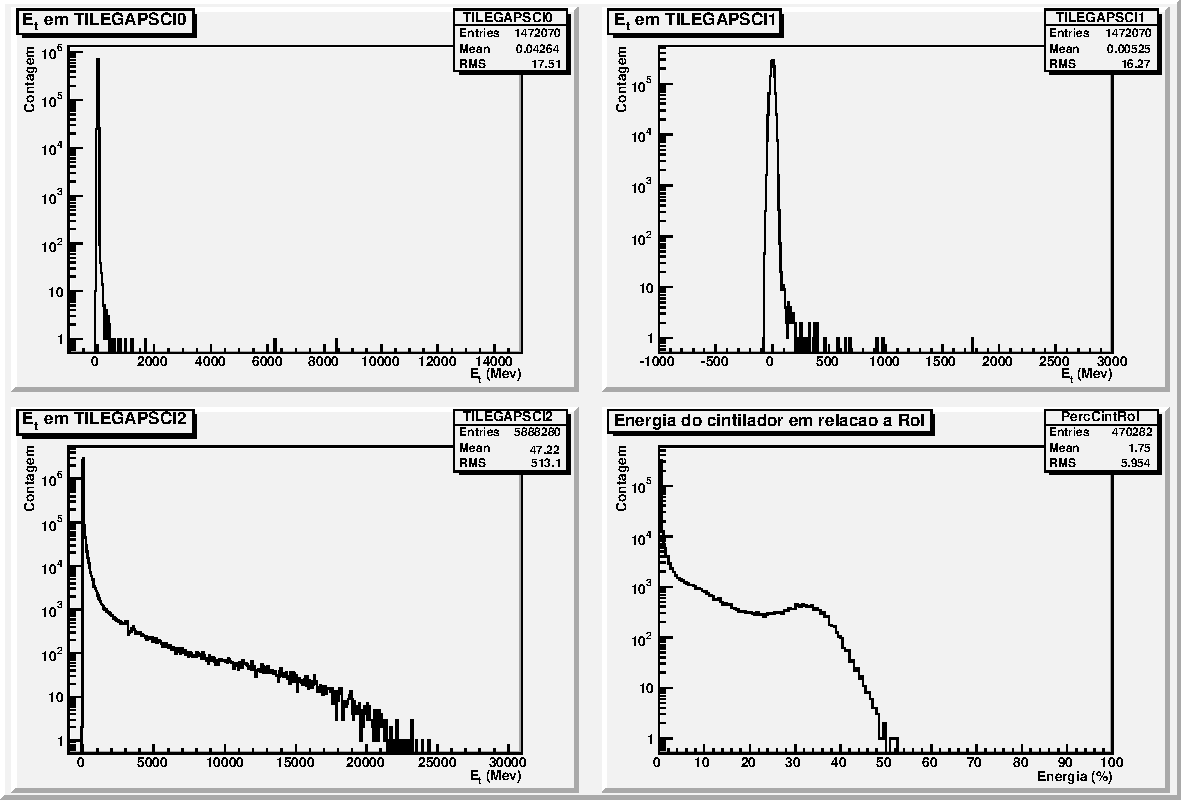
\includegraphics[height = 7cm]{histograma_energia_cintiladores_com_crack}
\caption{Deposição de energia no cintilador posicionado em $0,8 \leq | \eta | \leq 1,6$.} 
\label{fig:deposicao_energia_cintiladores} 
\end{figure} 

***DIZER QUE ESTES EVENTOS FORAM EXTRAIDOS DIRETAMENTE DO ATHENA, POR UM PACOTE NOSSO. FALAR COMO FUNCIONA ESSE PACOTE (NTUPLES, ETC)***

\section{Anelamento}

Os eventos validados na sessão~\ref{sec:geracao_eventos} possuem, como principal problema, dimensão elevada e não uniforme (vide figura~\ref{fig:distribuicao_numero_celulas_roi})

